\documentclass{article}

% Code syntax highlighting
% https://www.overleaf.com/learn/latex/Code_Highlighting_with_minted
\usepackage{minted}
\usemintedstyle{borland}

% If you're new to LaTeX, here's some short tutorials:
% https://www.overleaf.com/learn/latex/Learn_LaTeX_in_30_minutes
% https://en.wikibooks.org/wiki/LaTeX/Basics

% Formatting
\usepackage[utf8]{inputenc}
\usepackage[a4paper, margin=1in]{geometry}
\usepackage[titletoc,title]{appendix}
\usepackage{indentfirst}

% Math
% https://www.overleaf.com/learn/latex/Mathematical_expressions
% https://en.wikibooks.org/wiki/LaTeX/Mathematics
\usepackage{amsmath,amsfonts,amssymb,mathtools}
\DeclareMathOperator*{\argmax}{argmax} % thin space, limits underneath in displays


% Images
% https://www.overleaf.com/learn/latex/Inserting_Images
% https://en.wikibooks.org/wiki/LaTeX/Floats,_Figures_and_Captions
\usepackage{graphicx,float}
%Path relative to the main .tex file 
\graphicspath{ {./images/} }

% Tables
% https://www.overleaf.com/learn/latex/Tables
% https://en.wikibooks.org/wiki/LaTeX/Tables

% Algorithms
% https://www.overleaf.com/learn/latex/algorithms
% https://en.wikibooks.org/wiki/LaTeX/Algorithms
\usepackage[ruled,vlined]{algorithm2e}
\usepackage{algorithmic}


% Sections in a new page
\usepackage{titlesec}
\newcommand{\sectionbreak}{\clearpage}
\newcommand{\subsectionbreak}{\clearpage}

\usepackage{hyperref}


% Title content
\title{A0184594N}
\author{A0184594N}

\begin{document}

\section{Chapter 3 - Parallel Computing Platforms}

\subsection{Source of Processor Performance Gain}
Parallelism of various forms exist to have some performance gain
\begin{itemize}
    \item Single Processor
          \begin{itemize}
              \item Bit Level
                    \begin{itemize}
                        \item We don't processs bit by bit, but instead word by word.
                    \end{itemize}

              \item Instruction Level
                    \begin{itemize}
                        \item Pipelining (parallelism across time)
                              \begin{itemize}
                                  \item Split instruction into different stages
                                  \item allow multiple instructions to occupy different stages at same clock cycle.
                                  \item Number of pipeline stages == Maximum achievable speedup
                              \end{itemize}
                        \item Superscalar (parallelism across space)
                              \begin{itemize}
                                  \item Duplicate the pipelines
                                  \item Allow multiple instructions to pass through the same stage.
                                  \item Hard to schedule, find instructions that can be run together. (Dymanic - Hardware decision, Static - Compiler decision)
                                  \item Disadvantage: structural hazard
                              \end{itemize}
                        \item But is very limited, at most 2-3 instructions one time. due to data/control dependencies
                        \item Most CPUs have this. Usually we calculate Instructions per cycle, not Cycle-per-instruction.
                    \end{itemize}
              \item Thread Level
                    \begin{itemize}
                        \item Multithreading was originally a software mechanism
                        \item allow multiple parts of the same program to execute concurrently
                        \item Processor can provide hardware support for "thread context" like program counter and register (hyper-threading, etc..)
                        \item software threads can be executed in parallel
                    \end{itemize}
                    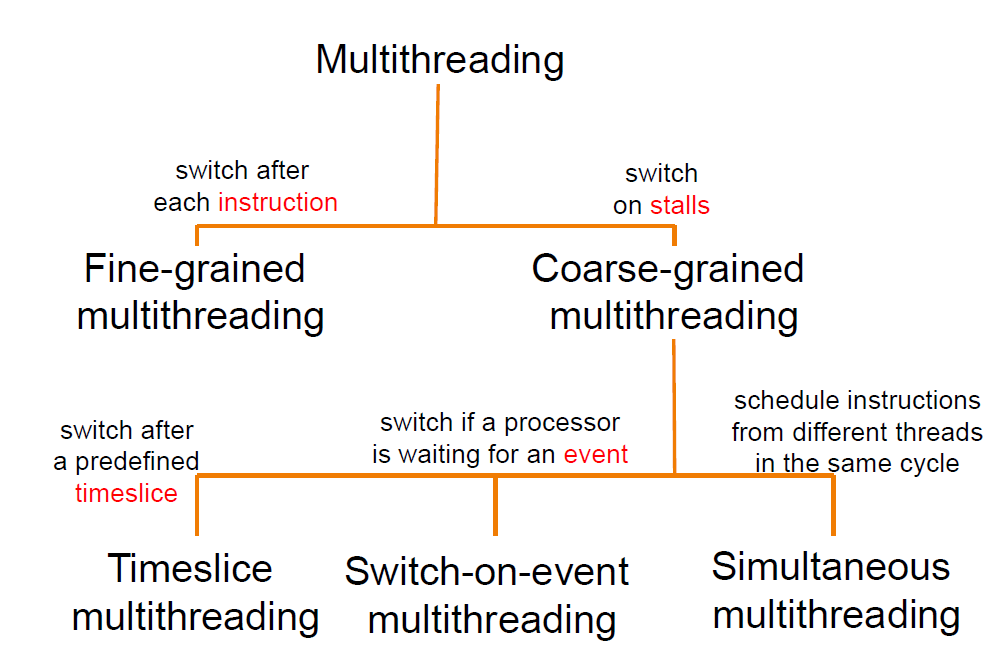
\includegraphics[width=0.7\textwidth]{l3_multithreading_implementation}
              \item Process Level
                    \begin{itemize}
                        \item Multiple processes work in parallel
                        \item independent memorry space, need special mechanism to communicate
                        \item Operating system provide IPC (Inter-Process communication) mechanism
                        \item Each process has independent context, can be mapped to multiple processor cores
                    \end{itemize}
          \end{itemize}
    \item Multi Processor
          \begin{itemize}
              \item Processor Level
                    \begin{itemize}
                        \item Shared Memory
                        \item Distributed Memory
                    \end{itemize}
          \end{itemize}
\end{itemize}

\subsection{Flynn's Parallel Architecture Taxonomty}
\begin{itemize}
    \item SISD (Single Instruction Single Data)
          \begin{itemize}
              \item A single instruction stream is executed
              \item Each instruction work on single data
              \item Most of the uniprocessor
          \end{itemize}
    \item SIMD (Single Instruction Multiple Data)
          \begin{itemize}
              \item A single stream of instructins
              \item Each instruction work on multiple data
              \item supercomputer during 1980s
              \item To exploit data parallelism, also known as vector processor
              \item Most modern processor has some form of SIMD
          \end{itemize}
    \item MISD (Multiple Instruction Single Data)
          \begin{itemize}
              \item Multiple stream of instructins
              \item All instruction work on same data at any time
              \item No actual implementaion, just here for completeness
          \end{itemize}
    \item MiMD (Multiple Instruction Multiple Data)
          \begin{itemize}
              \item Each Processing Unit fetch its own instruction
              \item Each Processing operates on its data
              \item Most popular model for multiprocessor
          \end{itemize}
\end{itemize}

Variant - SIMD and MIMD. nVidia GPUs have a set of threads executing the same code (SIMD) and multiple set of threads executing in parallel (MIMD)

\subsection{Multicore Architecture}
\subsubsection{Hierarchical design}
Multiple cores share multiple caches.
Cache size increase from the leaves to the root.
Found in comon day desktop, GPUs.

\subsubsection{Pipelined design}
Data elements are processed by multiple (different) execution cores in a pipelined way.
Bacuase same computation steps have to be applied to a long sequence of data elements.
Found in networking application, or GPUs.

\subsubsection{Network-based design}
Cores and their local caches and memories are connected via an interconnection network
Each core communicate with other cores / memory through this network.

\subsection{Memory Organization}
Memory can have consistency problem.
If one processor updates value in memory, How will other cores also update their values.
This also extends to the cache. Where we have cache coherence problem.
If we update value in the cache, how will other processor also update the same value in their caches.

2 Factors differentiate shared memory systems
\begin{itemize}
    \item Processor to Memory Delay (UMA/NUMA)
    \item presence of a local cache with cache coherence protocol (CC/NCC)
\end{itemize}

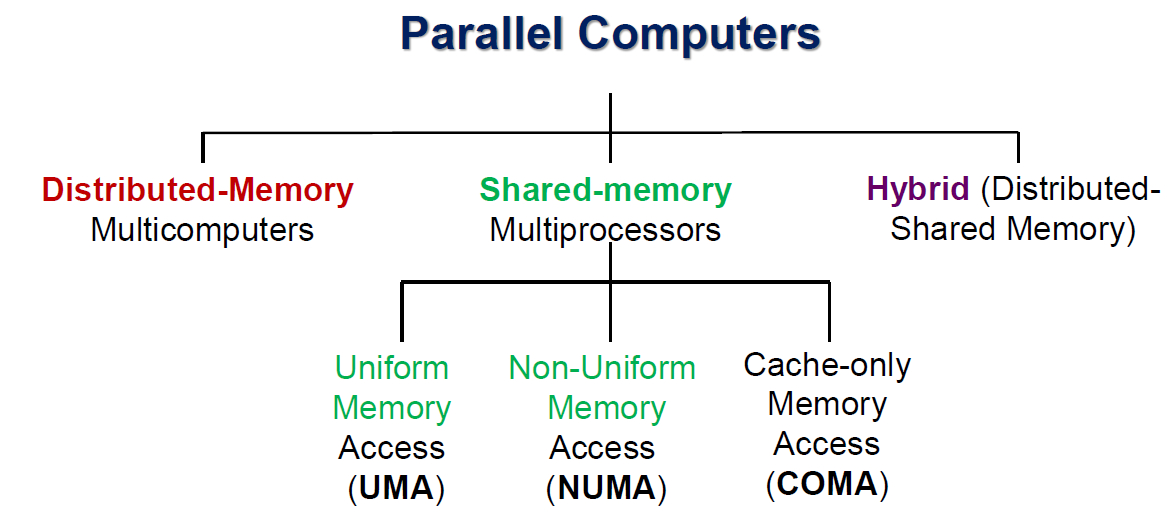
\includegraphics[width=0.9\textwidth]{l3_memory_organization}

\begin{itemize}
    \item Distributed Memory Systems
          \begin{itemize}
              \item Each node is independent, communicate with message passing
          \end{itemize}
          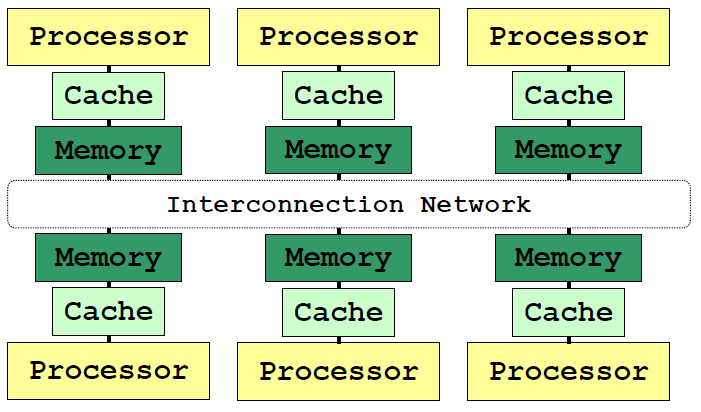
\includegraphics[width=0.9\textwidth]{l3_distributed_memory_system}
    \item Shared Memory
          \begin{itemize}
              \item Uniform Memory Access (Time) (UMA)
                    \begin{itemize}
                        \item Latency of accessing main memory is the same for each procesor
                        \item Good for low under of processors
                    \end{itemize}
                    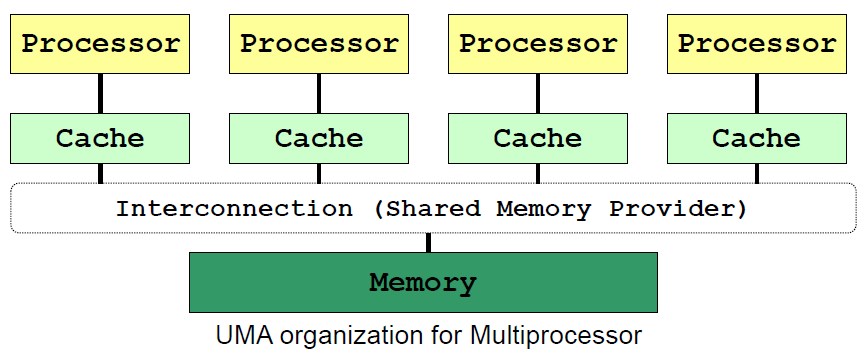
\includegraphics[width=0.9\textwidth]{l3_uniform_memory_access}
              \item Non-Uniform Memory Access
                    \begin{itemize}
                        \item Physically distributed memory of all processing elemets are combined to form a global shared memory
                        \item Processor can access local memory faster than remote memory
                    \end{itemize}
                    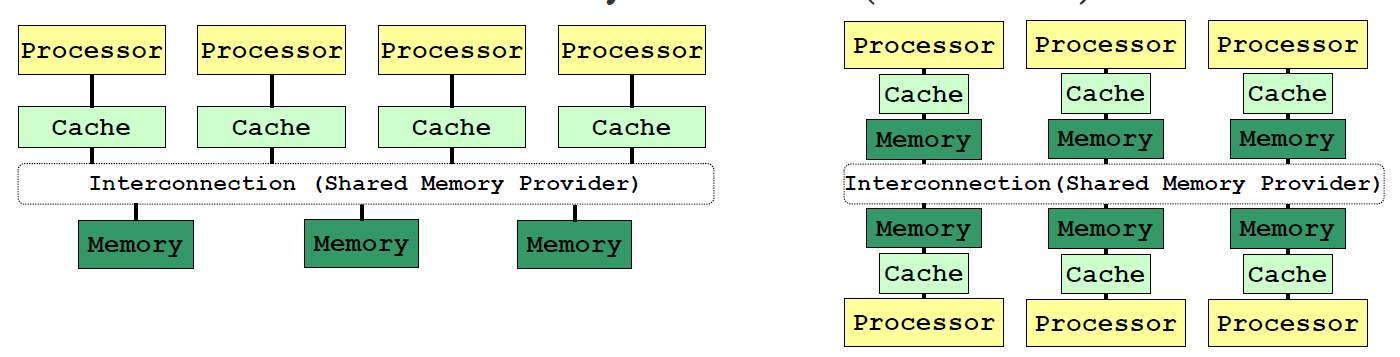
\includegraphics[width=0.9\textwidth]{l3_numa.png}
              \item Cache Coherent Non Uniform Memory Access (ccNUMA)
                    \begin{itemize}
                        \item Each node has cache to reduce contention
                    \end{itemize}
                    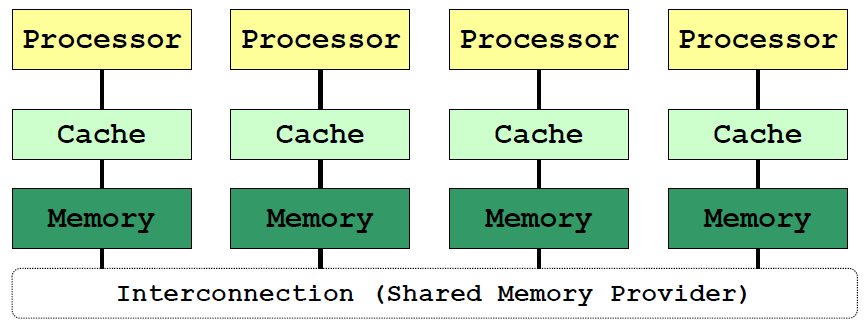
\includegraphics[width=0.9\textwidth]{l3_ccnuma.png}
              \item Cache Only Memory Architecture
                    \begin{itemize}
                        \item Each memory block works as cache memory
                        \item Uses cache coherence scheme to migrate datq
                    \end{itemize}
                    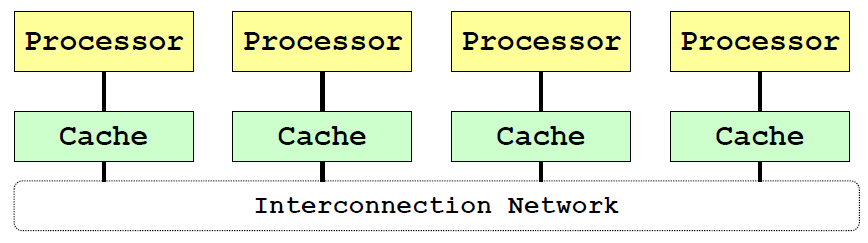
\includegraphics[width=0.9\textwidth]{l3_coma.png}
              \item Advantages
                    \begin{itemize}
                        \item No need to partition code or data
                        \item No need to physically move data among processors, there is effficient communication
                    \end{itemize}
              \item Disadvantages
                    \begin{itemize}
                        \item Special synchronization constructs are required
                        \item Lack of scalability due to contention
                    \end{itemize}
          \end{itemize}
    \item Hybird
          \begin{itemize}
              \item Servers, use shared among distributed
          \end{itemize}
\end{itemize}

\section{Chapter 4}

\end{document}
